%%%%%%%%%%%%%%%%%%%%%%%%%%%%%%%%%%%%%%%%%%%%%%%%%%%%%%%%%%%%%%%%%%%%%%%%%%%%%%%
% BAND ASSIGN
%%%%%%%%%%%%%%%%%%%%%%%%%%%%%%%%%%%%%%%%%%%%%%%%%%%%%%%%%%%%%%%%%%%%%%%%%%%%%%%
\begin{figure}
\centering
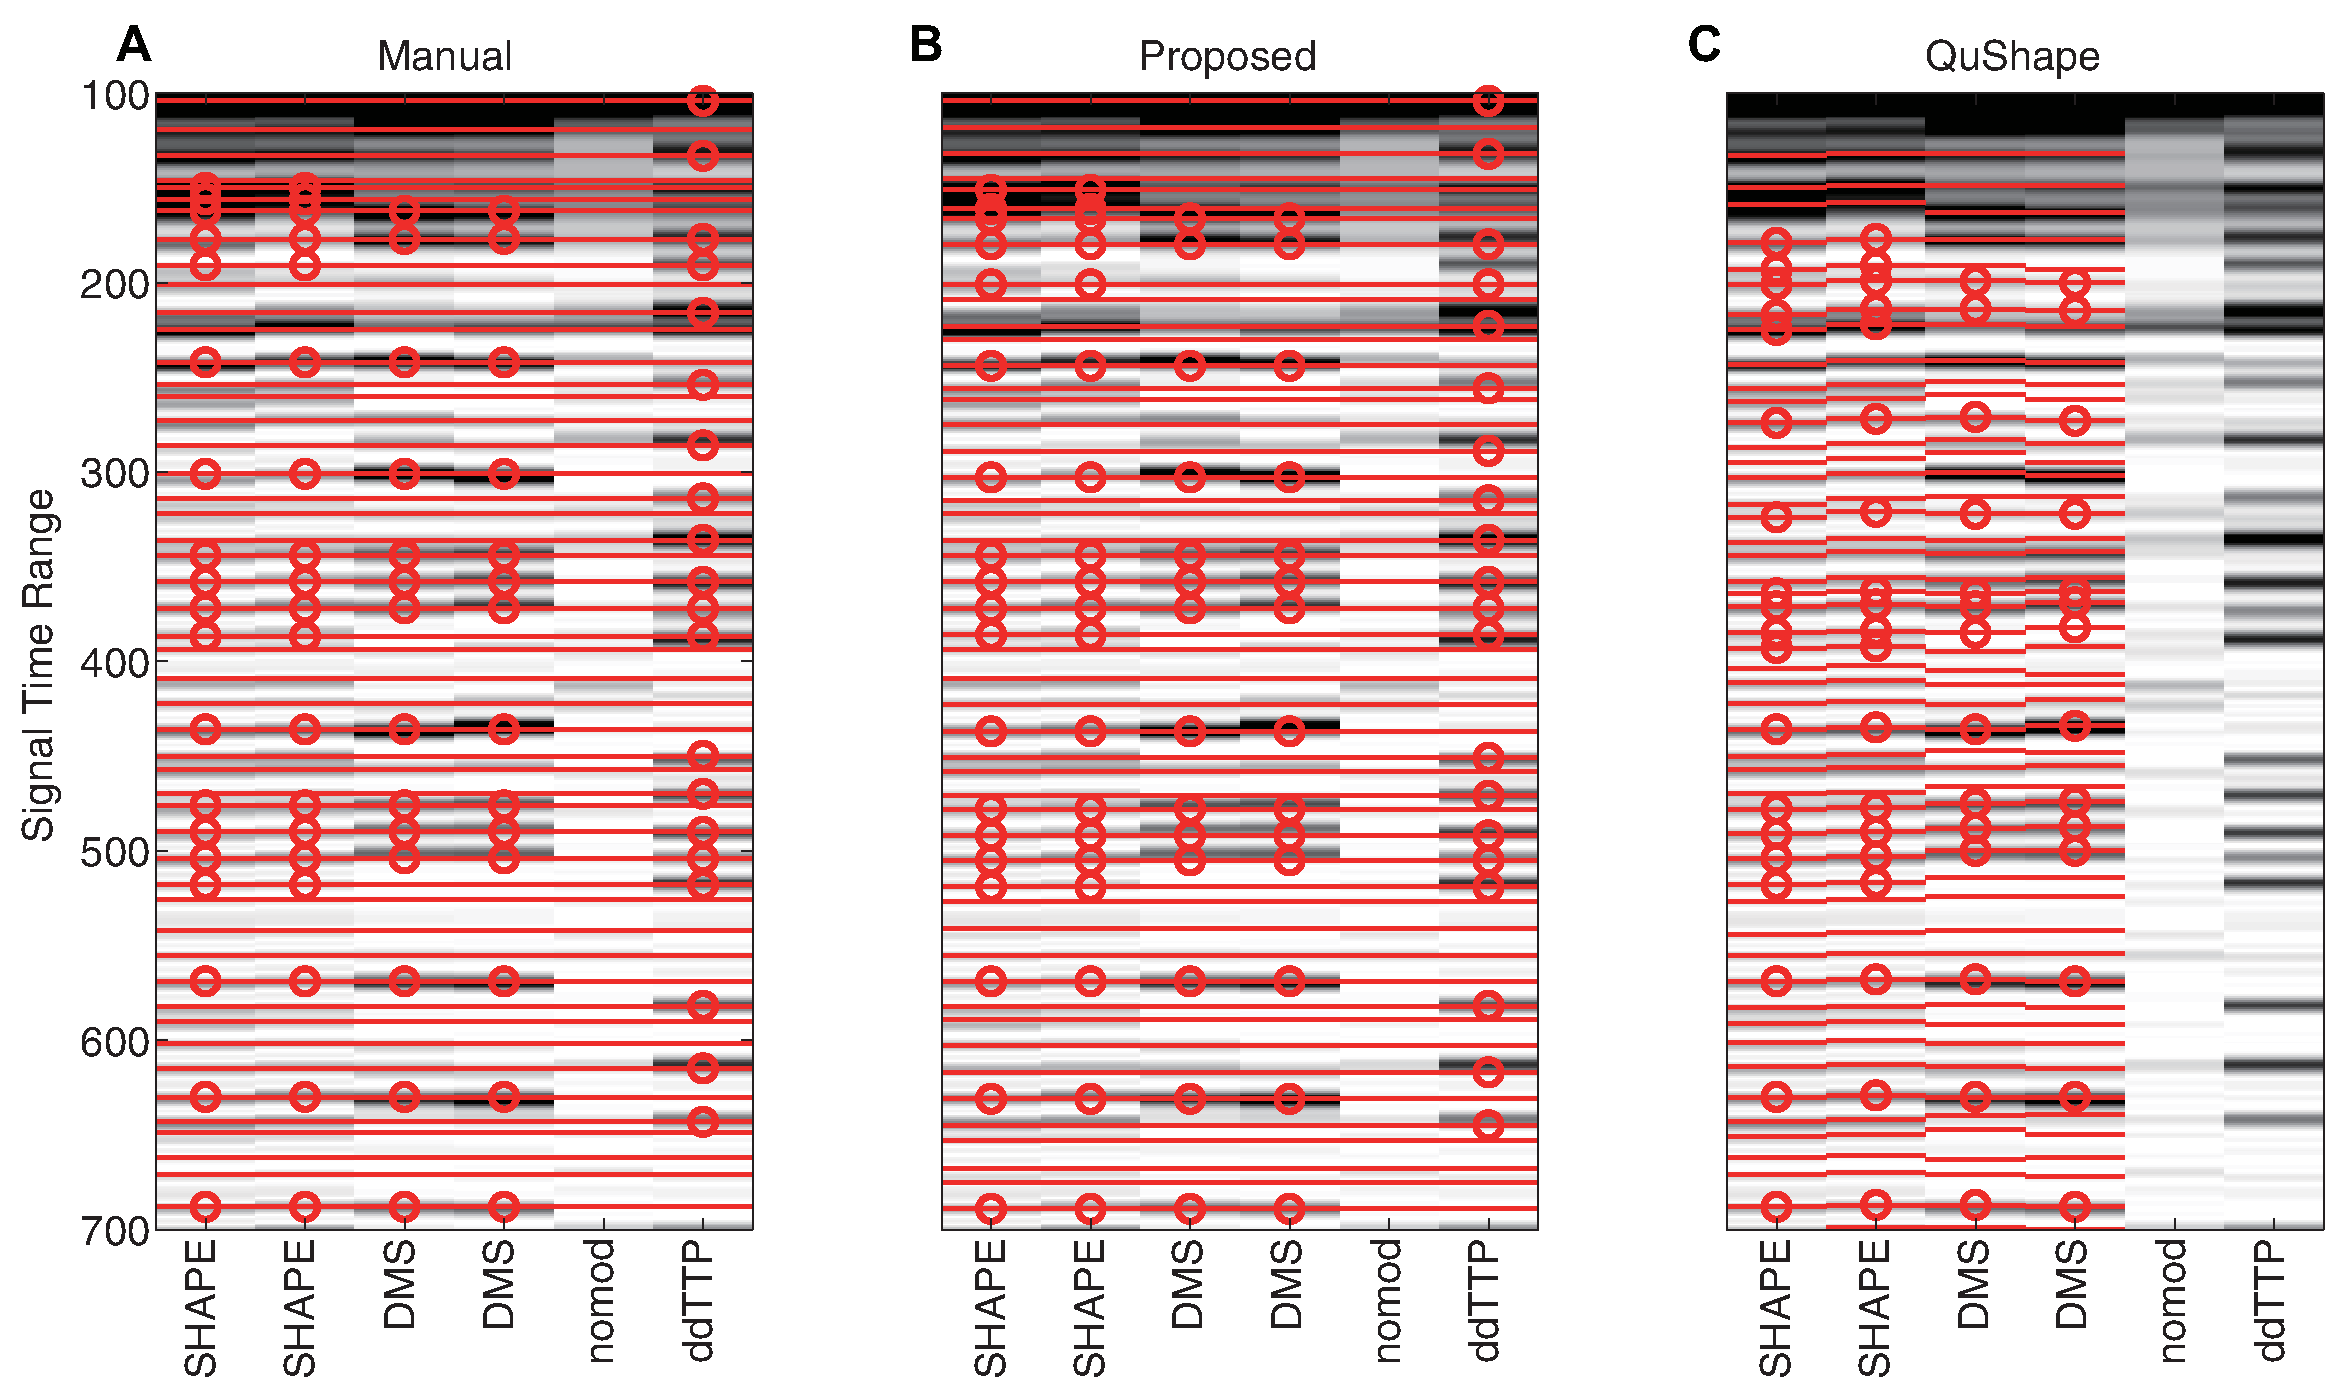
\includegraphics[width=0.9\linewidth]{figures/result_band_assign6}
\caption{Determination of band locations for data set `ViennaRNA design 03.' (\textbf{a}) Reference (manual) annotation. Red horizontal lines represent all determined locations corresponding to RNA sequence. Red circles represent band locations. (\textbf{b}) The band locations determined by the proposed method. (\textbf{c}) The band locations found by QuShape~\citep{Karabiber2013}.}
\label{f:band-assign}
\end{figure}
%%%%%%%%%%%%%%%%%%%%%%%%%%%%%%%%%%%%%%%%%%%%%%%%%%%%%%%%%%%%%%%%%%%%%%%%%%%%%%%

%%%%%%%%%%%%%%%%%%%%%%%%%%%%%%%%%%%%%%%%%%%%%%%%%%%%%%%%%%%%%%%%%%%%%%%%%%%%%%%
% BOX PLOTS
%%%%%%%%%%%%%%%%%%%%%%%%%%%%%%%%%%%%%%%%%%%%%%%%%%%%%%%%%%%%%%%%%%%%%%%%%%%%%%%
\begin{figure}
\centering
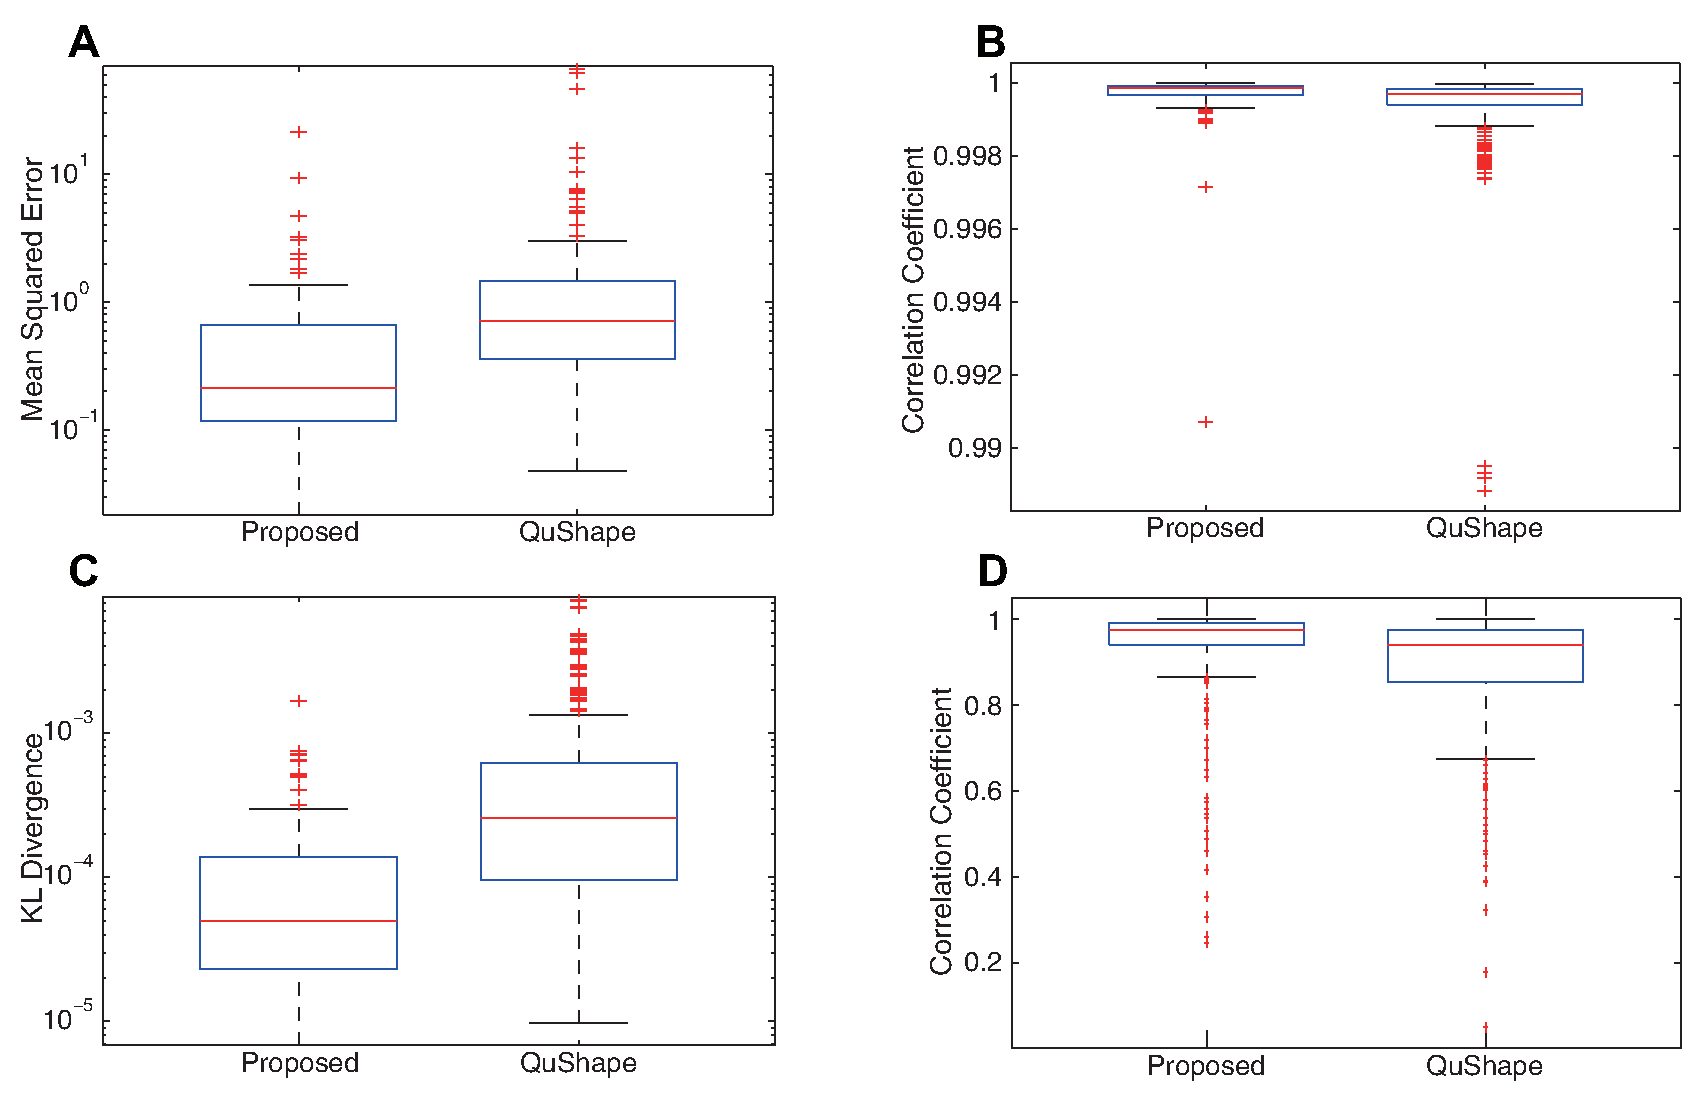
\includegraphics[width=0.9\linewidth]{figures/boxplots}
\caption{Proposed method (left) vs. QuShape (right). Each plot represents a certain distribution across 95 data sets. (\textbf{a}) Mean squared error (MSE) for band locations (\textbf{b}) Pearson's correlation coefficient for band locations (\textbf{c}) KL divergence for band locations (\textbf{d}) Pearson's correlation coefficients for area quantification. MSE units are normalized so that average distance between band locations is unity.}
\label{f:boxplots}
\end{figure}
%%%%%%%%%%%%%%%%%%%%%%%%%%%%%%%%%%%%%%%%%%%%%%%%%%%%%%%%%%%%%%%%%%%%%%%%%%%%%%%


\newcommand{\bP}{{\mathbf{P}}}

\subsection{Robust determination of band positions}\label{ss:band-position}
Figure~\ref{f:band-assign}(a)--(c) shows the electrophoretic profiles annotated with band locations by three different methods: reference, proposed, and QuShape~\citep{Karabiber2013}, respectively. The reference annotation was based on expert assignments carried out at the time of data acquisition~\citep{lee2014eterna} QuShape was chosen as the comparison target for its superior accuracy in band annotation relative to other software we tested, FAST and ShapeFinder (data not shown); nomod and ddTTP profiles were used as references (RXS1, BGS1) while running QuShape. Visual inspection suggests that the proposed method produces annotations more compatible with the reference. In this profile, the annotation determined by QuShape deviates from the reference position, particularly near the beginning of sequence.

To generally and quantitatively assess the accuracy of automated band annotation, we applied the proposed method and QuShape to 95 data sets acquired in the EteRNA project (Table \ref{t:data}). For both methods, we computed the mean squared error (MSE) of the band locations determined by the proposed method with respect to the reference locations, in units of average distance between locations. For a sense of scale, the typical MSE achieved by expert annotation is 0.15, based on comparisons of different experts' annotations with each other and to next-generation-sequencing-based measurements, where sequence annotation is unambiguous \citep{Kladwang2014}; see Supplemental Fig. S2. In our experience, a band annotation result with MSE lower than 0.5 typically requires no or a small number single-click corrections. The box plots in Figure~\ref{f:boxplots}(a)--(c) and individual MSE values (Supplemental Tables S1 and S2) reveal that the proposed method outperforms QuShape across the data sets. For example, the median MSE of the proposed method is 0.21, well under our target value of 0.5, compared to 0.72 from QuSHAPE. As separate metrics of accuracy, we measured the Pearson's correlation coefficient and the Kullback-Leibler (KL) divergence between the reference and computationally determined band positions.  Again, the average correlation coefficient of the proposed method is 1.68 times closer to 1, and the average KL divergence is 5.84 times smaller. These results quantitatively confirm what we observed qualitatively on using these tools: significantly less manual intervention is needed with the proposed method compared to QuShape.

%%%%%%%%%%%%%%%%%%%%%%%%%%%%%%%%%%%%%%%%%%%%%%%%%%%%%%%%%%%%%%%%%%%%%%%%%%%%%%%
% PEAK AREA
%%%%%%%%%%%%%%%%%%%%%%%%%%%%%%%%%%%%%%%%%%%%%%%%%%%%%%%%%%%%%%%%%%%%%%%%%%%%%%%
\begin{figure}
\centering
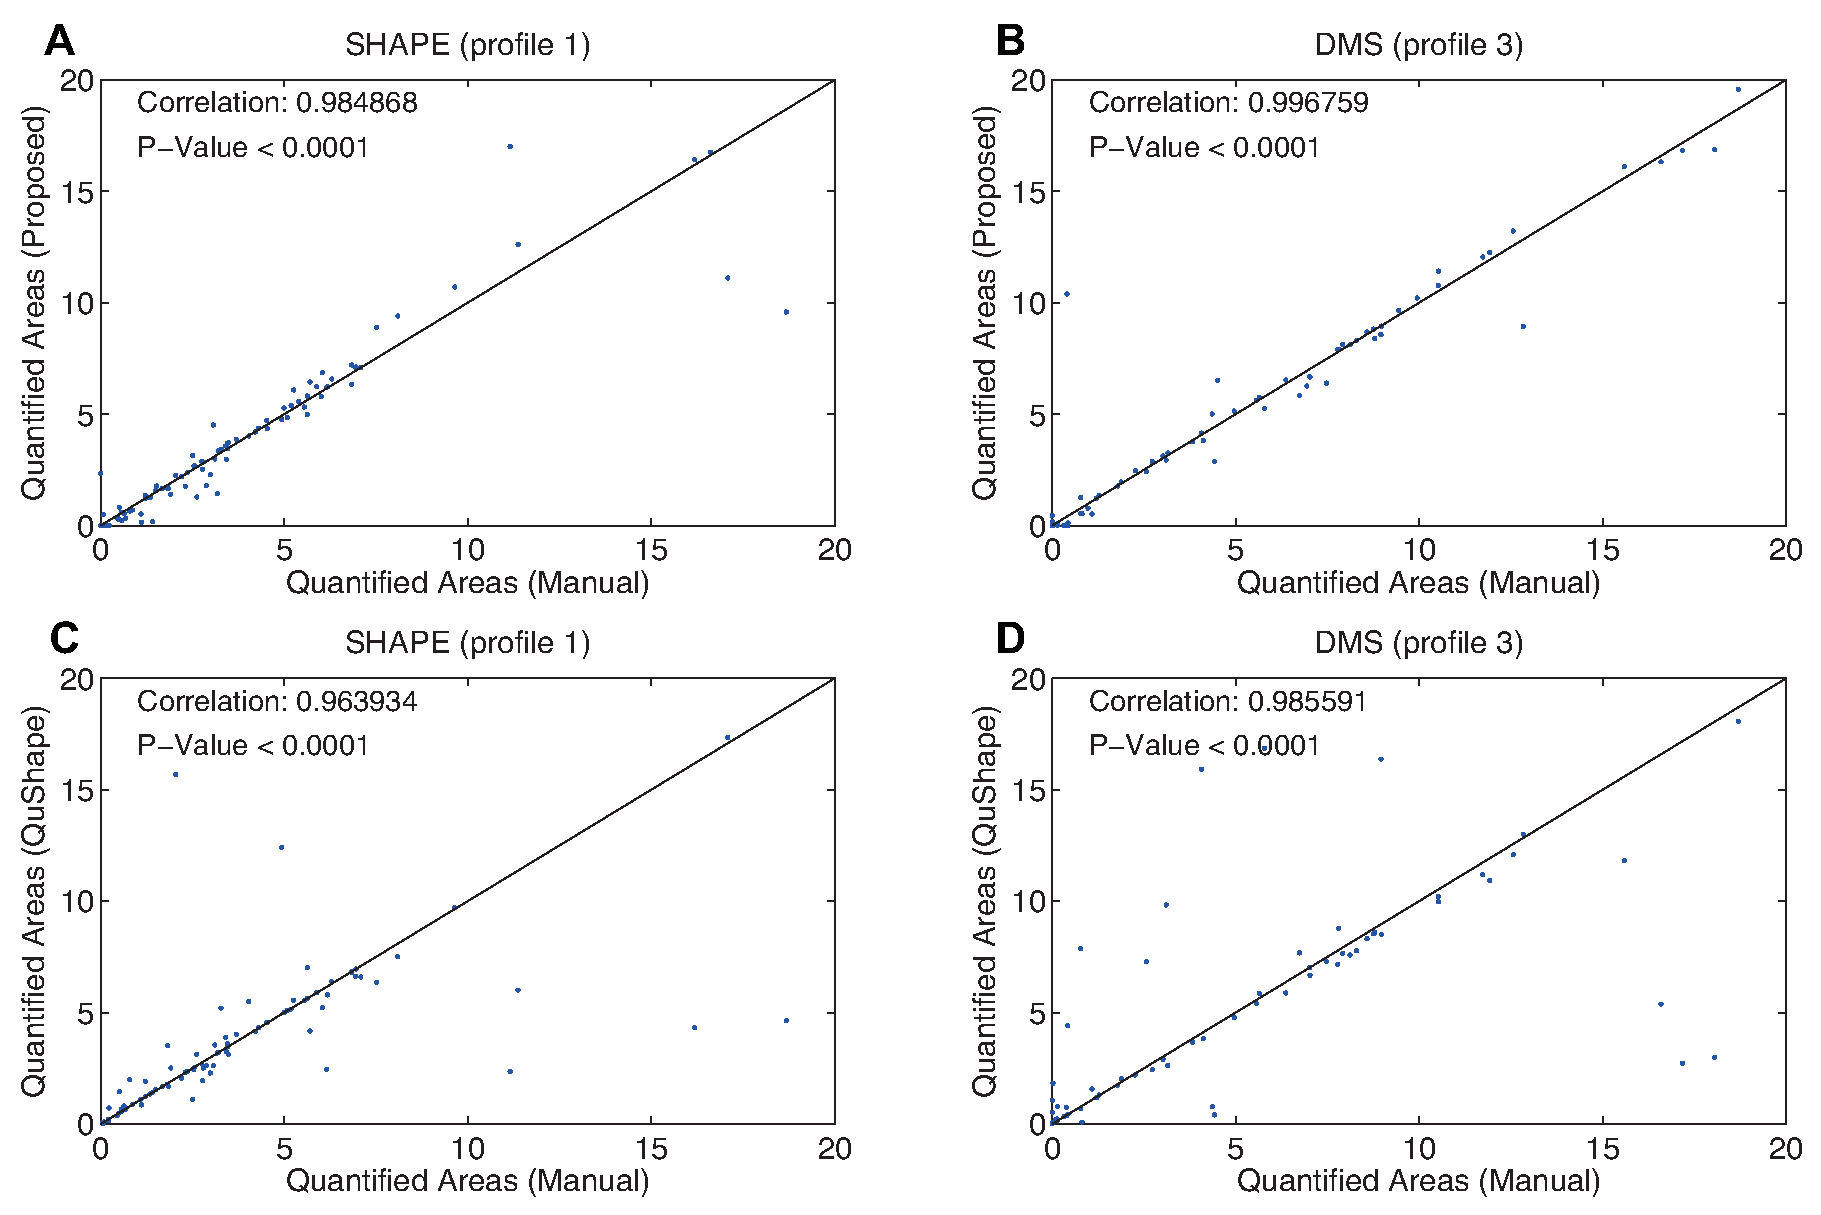
\includegraphics[width=0.9\linewidth]{figures/result_peak_area5}
\caption{Accuracy of quantifying peak areas for data set `FMN Binding Branches'. (\textbf{a}--\textbf{b}) Correlation of the reference and the quantified areas by the proposed method is shown for profiles 1 (SHAPE) and 3 (DMS). (\textbf{c}--\textbf{d}) Correlation of the reference and the areas quantified by QuShape.
}
\label{f:peak-area}
\end{figure}
%%%%%%%%%%%%%%%%%%%%%%%%%%%%%%%%%%%%%%%%%%%%%%%%%%%%%%%%%%%%%%%%%%%%%%%%%%%%%%%

\subsection{Accurate peak-area quantification}\label{ss:peak-area}
In the RNA structure mapping pipeline, the band annotation is followed by peak deconvolution, which fits each band with a Gaussian curve and outputs the quantified area of the band. To see how these final band quantification results are impacted by the band annotation method, we calculated Pearson's correlation coefficients between band areas quantified based on the band annotation found by the proposed method and those quantified based on the reference annotation. We also repeated the calculation with the band intensities quantified by QuShape. For fair comparison, we applied the same peak deconvolution software (HiTRACE; \citealp{Yoon2011}) to these three methods.

As one example, Figure~\ref{f:peak-area}(a)--(b) shows the correlation of results between the proposed method and reference for a specific data set (FMN Binding Branches) for two chemical modification strategies (SHAPE and DMS). Figure~\ref{f:peak-area}(c)--(d) shows the correlation between the QuShape and reference results, which is visually worse than the proposed method in both cases. Over all the data sets, Figure~\ref{f:boxplots}(d) and Supplemental Table S1 gives the distribution of the Pearson's correlation coefficients. The median correlation coefficient for the proposed method is 0.976, which is higher than that for QuShape (0.939) and the distribution for the proposed method shows smaller variance. This observation suggests that using the proposed band annotation can significantly enhance the accuracy of band quantification. 


%%%%%%%%%%%%%%%%%%%%%%%%%%%%%%%%%%%%%%%%%%%%%%%%%%%%%%%%%%%%%%%%%%%%%%%%%%%%%%%
% E-SCORE MSE
%%%%%%%%%%%%%%%%%%%%%%%%%%%%%%%%%%%%%%%%%%%%%%%%%%%%%%%%%%%%%%%%%%%%%%%%%%%%%%%
\begin{figure}
\centering
	\psfrag{x}[][][0.7]{$\escore$-score}
	\psfrag{y}[][][0.7]{$\escore=1$}
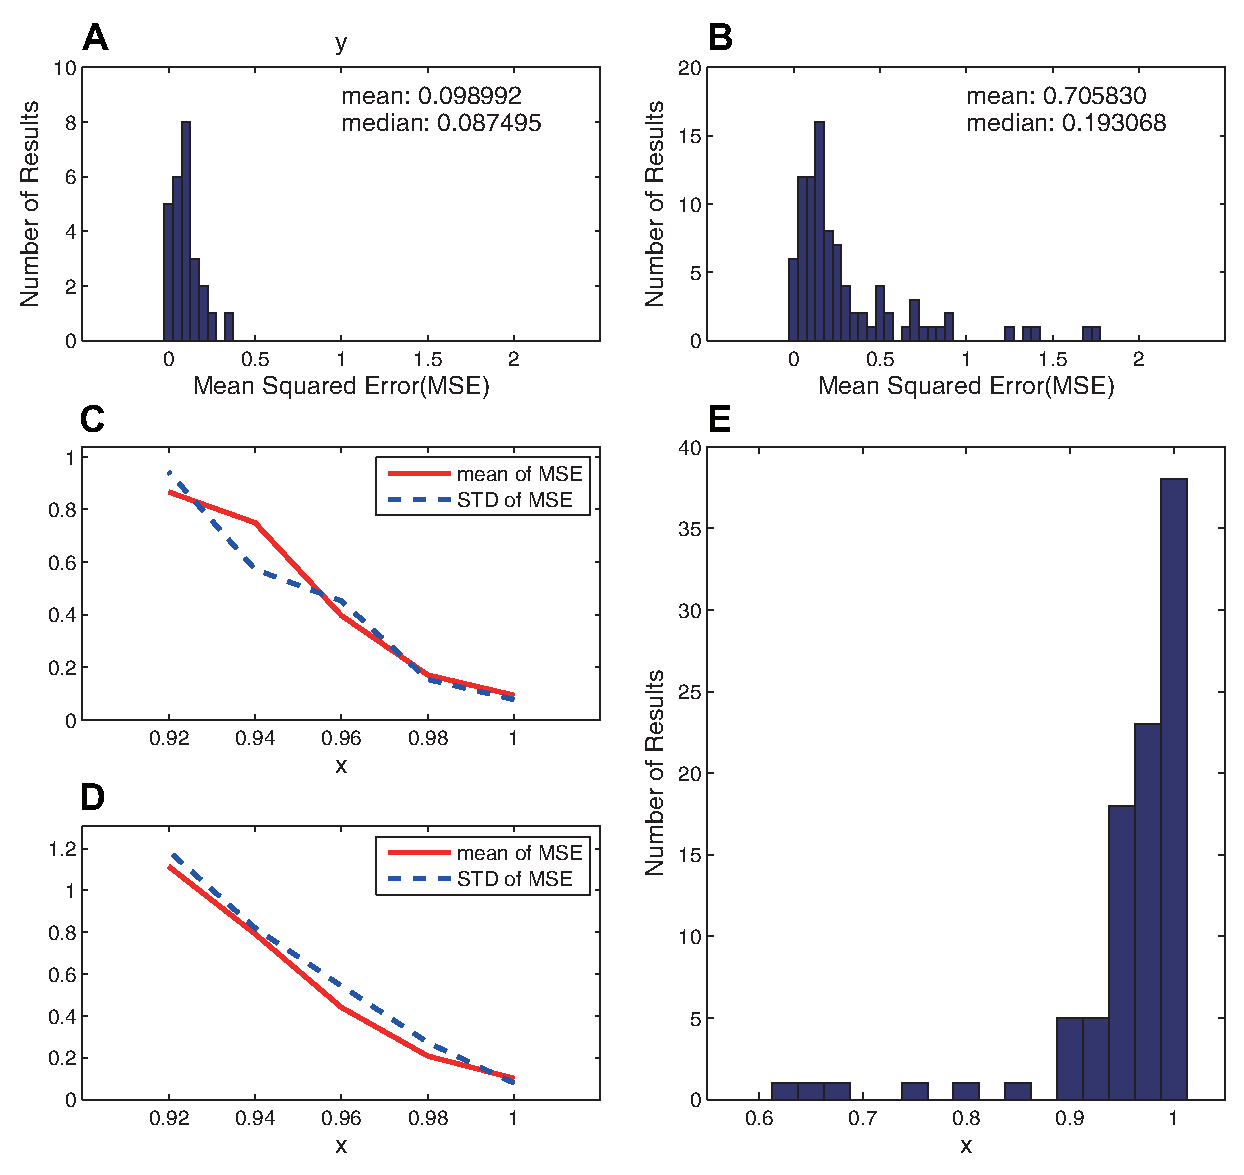
\includegraphics[width=0.9\linewidth]{figures/result_escore_mse4}
\caption{(\textbf{a}) Distribution of MSE for the results with 1 $\escore$-score. (\textbf{b}) Distribution of MSE for the whole 95 results. (5 results with MSE $> 2$ are ommited for better demonstration) (\textbf{c}) Trends of mean and standard deviation of MSE with respect to $\escore$-score over artificial data generated from a single original data set. (\textbf{d}) Trends of mean and standard deviation of MSE with respect to $\escore$-score for artificial data generated from the whole 95 data sets. (\textbf{e}) Distribution of $\escore$-score over 95 data sets.}
\label{f:escore-mse}
\end{figure}
%%%%%%%%%%%%%%%%%%%%%%%%%%%%%%%%%%%%%%%%%%%%%%%%%%%%%%%%%%%%%%%%%%%%%%%%%%%%%%%

\subsection{$\escore$-score reliability metric predicts MSE accuracy}

In Section~\ref{ss:reliability-evaluation}, we proposed $\escore$-score to evaluate the quality of results from our method. We assessed the use of $\escore$-score based on its ability to predict the accuracy of the band annotations compared to gold standard annotations, quantitatively evaluated as mean squared error (MSE). Figure~\ref{f:escore-mse}(a) show the distribution of the MSEs where (a) only contains results satisfying $\escore = 1.0$; the MSE values are substantially smaller than those in (b), which includes all 95 data sets.  For example, all 26 results under constraint $\escore=1.0$ have MSE below 0.5 as shown in (a), confirming that a `perfect' $\escore$-score essentially guarantees high quality of band annotations; furthermore, 50 out of 51 results with $\escore>0.97$ have MSE below 0.5 (even the one exception has MSE less than 1). In addition to this experimental test, artificial data sets were generated based on the original data sets through random convolution in terms of amplitude and interval for further verification. Figure~\ref{f:escore-mse}(c)--(d) show the trends of mean and standard deviation of MSE with respect to $\escore$-score, where (c) comes from artificial data generated from a single data set whereas artificial data involved in (d) is generated from the whole 95 data sets. The trends shown in (c) and (d) further confirm that a lower $\escore$-score corresponds to MSE values with higher (worse) mean and standard deviation. Figure~\ref{f:escore-mse}(e) shows the histogram of the $\escore$-scores over the 95 data sets prepared. Overall, 39\%  of the data sets have $\escore$-score equal to 1, and 84\%  have $\escore$-score greater than 0.97, suggesting that poor $\escore$-scores and subsequent detail manual correction will be encountered in a minority of cases.

\begin{comment}
%%%%%%%%%%%%%%%%%%%%%%%%%%%%%%%%%%%%%%%%%%%%%%%%%%%%%%%%%%%%%%%%%%%%%%%%%%%%%%%
% TABLE 2
%%%%%%%%%%%%%%%%%%%%%%%%%%%%%%%%%%%%%%%%%%%%%%%%%%%%%%%%%%%%%%%%%%%%%%%%%%%%%%%
\begin{table}
\processtable{Additional data sets and results from tests.
\label{t:additional_results}}
{\begin{tabular}{lcccc}
\toprule
Name & \# profiles & \# bands per profile & MSE & $\escore$-score \\
\midrule
GIR1 noref 	& 21 & 199 & 0.09 & 0.99 \\
GIR1 ref 		& 21 & 225 & 0.12 & 0.98 \\
AdoCbl noref 	& 16 & 179 & 0.61 & 0.97 \\
AdoCbl ref 	& 16 & 205 & 0.68 & 0.90 \\
VS noref 		& 48 & 195 & 0.16 & 0.96 \\
VS ref 		& 48 & 233 & 0.12 & 0.96 \\
SAM noref 	& 32 & 103 & 0.09 & 0.96 \\
SAM ref 		& 32 & 143 & 0.09 & 0.96 \\
HTP noref 	& 32 & 79  & 0.05 & 1.00 \\
HTP ref 		& 32 & 116 & 0.05 & 1.00 \\
Tbox 		& 20 & 141 & 0.34 & 0.98 \\
tRNA 		& 20 & 119 & 0.63 & 0.83 \\
cdiAMP 		& 36 & 171 & 0.16 & 0.99 \\
16S 			& 8  & 125 & 0.21 & 0.98 \\
C19 			& 16 & 319 & 0.18 & 0.99 \\
tC19 		& 16 & 248 & 0.01 & 1.00 \\
tC19Z 		& 16 & 248 & 0.01 & 0.99 \\
C1Lig 		& 7  & 167 & 0.04 & 1.00 \\
Hox5 		& 9  & 261 & 0.11 & 0.99 \\
Hox9D 		& 16 & 296 & 0.44 & 0.99 \\
L-21			& 20 & 413 & 2.00$^a$ & 0.98 \\
\botrule
\end{tabular}}
{$^a$An extraordinary result mainly caused by a misalignment between profiles (to be discussed in the discussion section) 
}
\end{table}
%%%%%%%%%%%%%%%%%%%%%%%%%%%%%%%%%%%%%%%%%%%%%%%%%%%%%%%%%%%%%%%%%%%%%%%%%%%%%%%
\end{comment}

\subsection{Results in longer, biological RNA sequences}
In an effort to test the proposed method's compatibility with a wide array of high-throughput RNA structure mapping data sets, we prepared sample experimental data sets of biologically derived RNAs. These additional 21 data sets include Class I ligase ~\citep{Bagby01122009}, the Tetrahymena L-21 ScaI ribozyme ~\citep{russell2006}, a four-way junction from the E. coli 16S ribsomal RNA ~\citep{tian2014nature}, RNA replicases (C19, tC19 and tC19Z) ~\citep{Wochner08042011}, human Hox transcripts $5^\prime$ UTR (Hox5 and Hox9D189) ~\citep{xue2014} and RNA Puzzle entries (\#5-10, and 12) ~\citep{Cruz01042012}. In each data set, complete sets of chemical modifier reactions (nomod, SHAPE, DMS, CMCT) and reference ladders (ddNTPs) are present. In addition, a hepatitis delta virus genomic segment studied previously allowed direct comparison to the FAST software (Supplemental Fig. S3) \citep{Pang2011}. These RNAs had lengths up to 400 nucleotides, significantly longer than the ~100-nt EteRNA designs (Table \ref{t:data}). Despite this increase in length, the band annotation results from the proposed method were still highly consistent with the reference expert annotation. Excluding an abnormal result from L-21 caused by an experimental issue that disallowed alignment of sequencing ladders, the maximum of MSE is only 0.68. Furthermore, the two worst MSE values (0.68 and 0.63) and two lowest $\escore$-scores (0.83 and 0.90) coincide in the results for AdoCbl(noref) and tRNA, confirming $\escore$-score's utility. 

\begin{comment}
%%%%%%%%%%%%%%%%%%%%%%%%%%%%%%%%%%%%%%%%%%%%%%%%%%%%%%%%%%%%%%%%%%%%%%%%%%%%%%%
% REACTIVITY COMPARISON
%%%%%%%%%%%%%%%%%%%%%%%%%%%%%%%%%%%%%%%%%%%%%%%%%%%%%%%%%%%%%%%%%%%%%%%%%%%%%%%
\begin{figure}
\centering
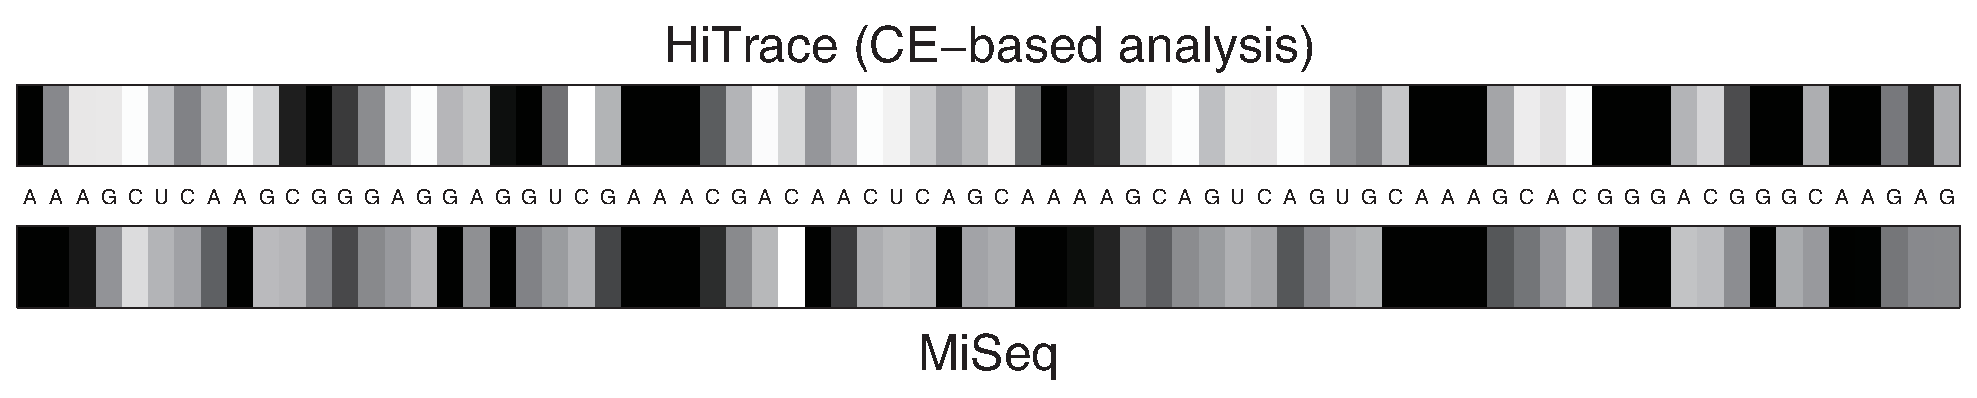
\includegraphics[width=\linewidth]{figures/reactivities}
\caption{Heatmaps those represent the reactivity values obtained by CE-based analysis and MiSeq, respectively. The data set used is 'C-BACK' sequence.}
\label{f:reactivity-comparison}
\end{figure}
%%%%%%%%%%%%%%%%%%%%%%%%%%%%%%%%%%%%%%%%%%%%%%%%%%%%%%%%%%%%%%%%%%%%%%%%%%%%%%%

\subsection{Reactivity comparison with miseq}
For the final step of verification, we compared the reactivity data obtained by using the proposed method in conjunction with HiTrace, with that obtained by using MiSeq method. In spite of their separated experimental samples and environments, the two reactivity data sets share a same trend as shown in Figure~\ref{f:reactivity-comparison}, evidencing the consistency between the two distinct analyses in terms of their final results.

\end{comment}
